\providecommand{\main}{../..}
\documentclass[\main/thesis.tex]{subfiles}
\begin{document}

\section{Converting from Natural Numbers}\label{fromnat}

\lstinline|Numeral| is a family of types, so are functions that are defined on
\lstinline|Numeral|.
It is important to regard functions such as \lstinline|⟦_⟧| as a collective;
each has a different configuration of indices.

Here, we name the function that converts natural numbers to corresponding
numerals \lstinline|fromℕ|.

\begin{figure}[H]
    \centering
    \begin{tikzpicture}
        \matrix (m) [matrix of nodes,row sep=6em,column sep=8em,minimum width=4em]
            {
                {\lstinline|Numeral b d o|} & {\lstinline|ℕ|} \\
            };
        \path[-stealth]
            ($(m-1-1.east)+(0,+0.1)$)
                edge node [above] {\lstinline|⟦_⟧|}
                ($(m-1-2.west)+(0,+0.1)$)
            ($(m-1-2.west)+(0,-0.1)$)
                edge node [below] {\lstinline|fromℕ|}
                ($(m-1-1.east)+(0,-0.1)$)
            ;
    \end{tikzpicture}
\caption{Converting between natural numbers and numerals}
\label{figure:31}
\end{figure}

Because \lstinline|fromℕ| should behave like an inverse function of \lstinline|⟦_⟧|,
the codomain of \lstinline|⟦_⟧| should be the domain of \lstinline|fromℕ|.
For \lstinline|fromℕ| to be well-defined, its corresponding \lstinline|⟦_⟧|
must be surjective.
However, not all instances of \lstinline|⟦_⟧| are surjective.

Take the numeral system \lstinline|Numeral 10 5 0| for example.
Natural numbers such as $ 5 $ or $ 6 $ cannot be converted to
\lstinline|Numeral 10 5 0| because its evaluation function \lstinline|⟦_⟧|
is not surjective.

\begin{figure}[H]
    \centering
    \begin{adjustbox}{max width=\textwidth}
        \begin{tikzpicture}

            % the frame
            \path[clip] (-6, -3) rectangle (15, 1.5);

            % the body
            \foreach \i in {0,...,1} {
                \foreach \j in {0,...,4} {
                    \draw[ultra thick, fill=white] ({\i*10+\j+0.05}, -0.2) rectangle ({\i*10+\j+0.95}, 0.2);
                    \path[->, ultra thick] ({\i*10+\j + 0.5}, -1.8) edge node {} ({\i*10+\j + 0.5}, -0.3);
                };
            }

            % nat
            \foreach \i in {0,...,15} {
                \draw[ultra thick, fill=black] ({\i+0.05}, -2) rectangle ({\i+0.95}, -1.9);
            }

            % label
            \foreach \i in {0,...,3} {
                \pgfmathsetmacro{\j}{int(\i * 5)}
                \node[below, scale=1.2] at ({\j+0.5}, -2) {\j};
            }

            \node[scale=1.5] at (-3, 0) {\lstinline|Numeral 10 5 0|};
            \node[scale=1.5] at (-3, -2) {\lstinline|ℕ|};
        \end{tikzpicture}
    \end{adjustbox}
\caption{Not all systems are surjective}
\label{figure:32}
\end{figure}

\subsection{Domains of \lstinline|fromℕ|}

We can define \lstinline|fromℕ| only on a subset of \lstinline|Numeral| that
possess surjective evaluation functions.
For a system to be surjective, in addition of being continuous, its numerals
would also have to be able to cover every natural number, including ``0''.

\begin{figure}[H]
    \centering
    \begin{adjustbox}{max width=\textwidth}
        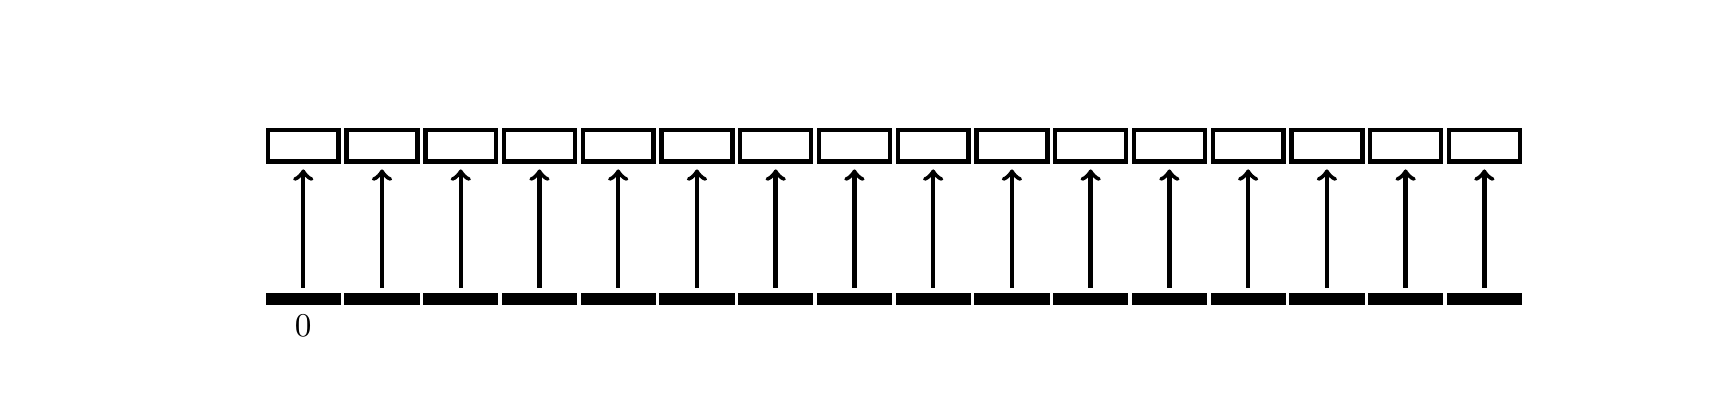
\begin{tikzpicture}

            % the frame
            \path[clip] (-3, -3) rectangle (18, 1.5);

            % the body
            \foreach \i in {0,...,15} {
                \draw[ultra thick, fill=white] ({\i+0.05}, -0.2) rectangle ({\i+0.95}, 0.2);
                \path[->, ultra thick] ({\i + 0.5}, -1.8) edge node {} ({\i+ 0.5}, -0.3);
            };

            % nat
            \foreach \i in {0,...,15} {
                \draw[ultra thick, fill=black] ({\i+0.05}, -2) rectangle ({\i+0.95}, -1.9);
            }

            % label
            \node[below, scale=1.2] at (0.5, -2) {$0$};
        \end{tikzpicture}
    \end{adjustbox}
\caption{Surjective evaluation}
\label{figure:33}
\end{figure}


Therefore, the index $o$ can only be $0$ because that is where the least
numeral starts counting from. We can convert all natural numbers to such systems
by induction and recursively replacing the successor of \lstinline|ℕ| with
\lstinline|1+|.

\begin{lstlisting}
fromℕ : ∀ {b d}
    → {cont : True (Continuous? b (suc d) 0)}
    → ℕ
    → Numeral b (suc d) 0
fromℕ zero                  = z ∙
fromℕ {cont = cont} (suc n) = 1+ {cont = cont} (fromℕ n)
\end{lstlisting}

However, it would be a shame if only a few of \lstinline|Numeral| can be
converted from natural numbers, and all that effort we have put into
generalizing $ o $ will be gone to waste.

If we make \lstinline|fromℕ| a partial function, allowing it to convert only
a subset of natural numbers that are greater than $ o $ instead of $ 0 $,
then much more numeral systems will be applicable for \lstinline|fromℕ|.

\begin{figure}[H]
    \centering
    \begin{adjustbox}{max width=\textwidth}
        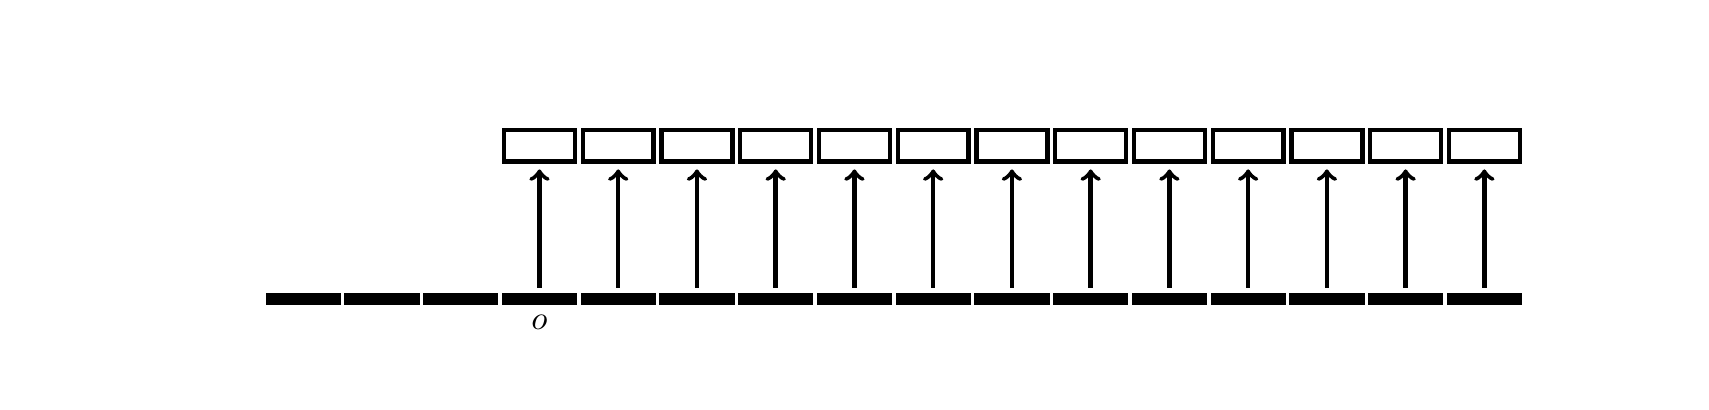
\begin{tikzpicture}

            % the frame
            \path[clip] (-3, -3) rectangle (18, 1.5);

            % the body
            \foreach \i in {3,...,15} {
                \draw[ultra thick, fill=white] ({\i+0.05}, -0.2) rectangle ({\i+0.95}, 0.2);
                \path[->, ultra thick] ({\i + 0.5}, -1.8) edge node {} ({\i+ 0.5}, -0.3);
            };

            % nat
            \foreach \i in {0,...,15} {
                \draw[ultra thick, fill=black] ({\i+0.05}, -2) rectangle ({\i+0.95}, -1.9);
            }

            % label
            \node[below, scale=1.2] at (3.5, -2) {$o$};

        \end{tikzpicture}
    \end{adjustbox}
\caption{``Partially surjective'' evaluation}
\label{figure:34}
\end{figure}


Besides, functions and predicates such as \lstinline|+1| and
\lstinline|Continuous| will still be useful;
we did not work our head off constructing these things for nothing.

We generalize the previous definition of \lstinline|fromℕ| and make $ o $ the
lower bound of the given \lstinline|ℕ|.
If the given number $ n $ happens to be equal to $ o $ then we return the least
numeral \lstinline|z ∙|, else we replace the successor with \lstinline|+1|
recursively by induction on $ n $.

\begin{lstlisting}
fromℕ : ∀ {b d o}
    → {cont : True (Continuous? b (suc d) o)}
    → (n : ℕ)
    → n ≥ o
    → Numeral b (suc d) o
fromℕ {o = o}       n       p   with o ≟ n
fromℕ               n       n≥o | yes eq = z ∙
fromℕ {o = o}       zero    n≥o | no ¬eq
    = contradiction (≤0⇒≡0 o n≥o) ¬eq
fromℕ {cont = cont} (suc n) n≥o | no ¬eq
    = 1+
        {cont = cont}
        (fromℕ {cont = cont} n (≤-pred (≤∧≢⇒< n≥o ¬eq)))
\end{lstlisting}

The domain we have chosen for \lstinline|fromℕ| seems reasonable.
However, there are other possible choices of the domain.

\subsection{Other options of the domain of \lstinline|fromℕ|}

Consider \lstinline|Numeral 1 1 2|, a unary system with only one digit
that is ``2''.

\begin{figure}[H]
    \centering
    \begin{adjustbox}{max width=\textwidth}
        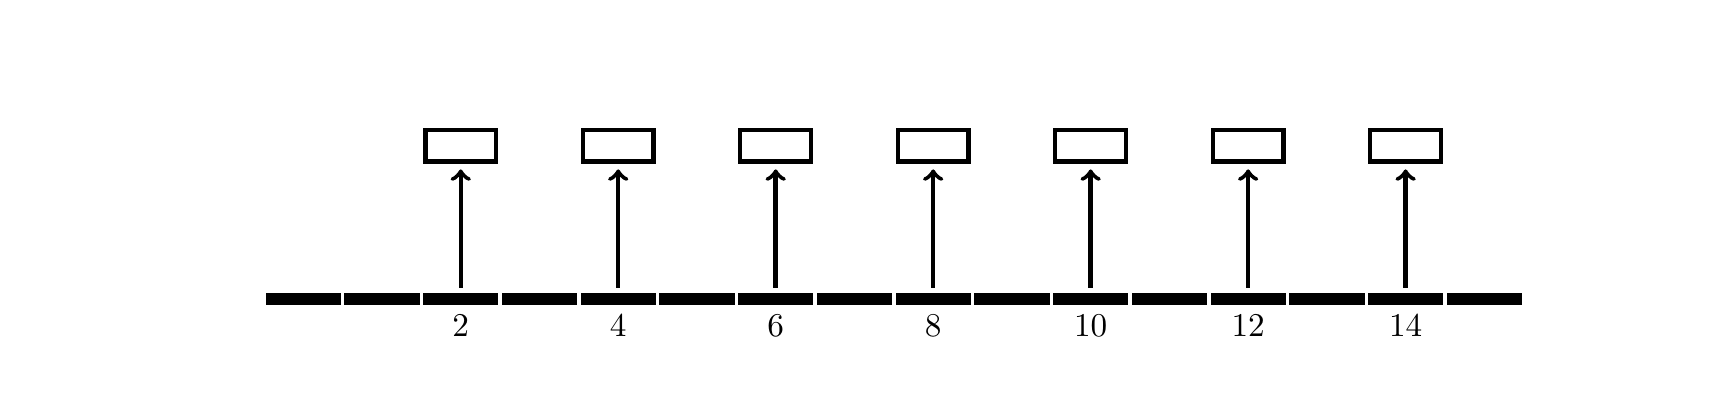
\begin{tikzpicture}

            % the frame
            \path[clip] (-3, -3) rectangle (18, 1.5);

            % the body
            \foreach \i in {1,...,7} {
                \pgfmathsetmacro{\j}{int(\i * 2)}
                \draw[ultra thick, fill=white] ({\i*2+0.05}, -0.2) rectangle ({\i*2+0.95}, 0.2);
                \path[->, ultra thick] ({\i*2 + 0.5}, -1.8) edge node {} ({\i*2+ 0.5}, -0.3);
                \node[below, scale=1.2] at ({\i*2+0.5}, -2) {\j};
            };

            % nat
            \foreach \i in {0,...,15} {
                \draw[ultra thick, fill=black] ({\i+0.05}, -2) rectangle ({\i+0.95}, -1.9);
            }
        \end{tikzpicture}
    \end{adjustbox}
\caption{Other kinds of domain}
\label{figure:35}
\end{figure}

Such a numeral system can represent all even numbers except for zero.
To convert natural numbers to \lstinline|Numeral 1 1 2|, we can devise a
predicate like \lstinline|Even-but-not-zero| such that only these numbers fit.

\begin{lstlisting}
fromℕ : ∀ {b d o}
    → (n : ℕ)
    → (Even-but-not-zero n)
    → Numeral b (suc d) o
\end{lstlisting}

In fact, we can even generalize from \lstinline|Numeral 1 1 1|
(ordinary unary numerals) and \lstinline|Numeral 1 1 2| to \lstinline|Numeral 1 1 n|
to describe all cyclic groups of order $ n $.

What about other kinds of predicates? Can we choose any subset of natural numbers
to convert from as long as it fits the targeting numeral system?
The point is, the reason why we choose a subset of natural numbers as the domain
of \lstinline|fromℕ| is \textbf{arbitrary} and \textbf{empirical}.

Nonetheless, we settled for this specific kind of \lstinline|fromℕ| because we
think that it can best describe the numerals that are closed under the successor
function and even the addition function, which may be suitable for indexing
numerical representations that supports operations such as insertion and merge.

\begin{lstlisting}
fromℕ : ∀ {b d o}
    → {cont : True (Continuous? b (suc d) o)}
    → (n : ℕ)
    → n ≥ o
    → Numeral b (suc d) o
\end{lstlisting}

\subsection{Properties of \lstinline|fromℕ|}

The property below states that \lstinline|fromℕ| is a \textit{right inverse} of
\lstinline|⟦_⟧|. Having a right inverse means that \lstinline|⟦_⟧| is
\textit{surjective}.

\begin{lstlisting}
fromℕ-toℕ : ∀ {b d o}
    → (cont : True (Continuous? b (suc d) o))
    → (n : ℕ)
    → (n≥o : n ≥ o)
    → ⟦ fromℕ {cont = cont} n n≥o ⟧ ≡ n
fromℕ-toℕ {o = o} cont n       n≥o with o ≟ n
fromℕ-toℕ         cont n       n≥o | yes eq = eq
fromℕ-toℕ {o = o} cont zero    n≥o | no ¬eq
    = contradiction (≤0⇒≡0 o n≥o) ¬eq
fromℕ-toℕ         cont (suc n) n≥o | no ¬eq =
    let
        n≥o' = ≤-pred (≤∧≢⇒< n≥o ¬eq)
    in
    begin
        ⟦ 1+ {cont = cont} (fromℕ {cont = cont} n n≥o') ⟧
    ≡⟨ 1+-toℕ {cont = cont} (fromℕ {cont = cont} n n≥o') ⟩
        suc ⟦ fromℕ {cont = cont} n n≥o' ⟧
    ≡⟨ cong suc (fromℕ-toℕ cont n n≥o') ⟩
        suc n
    ∎
\end{lstlisting}

Conversely, \lstinline|⟦_⟧| would also have a \textit{left inverse} if it is
injective.
However, \lstinline|⟦_⟧| would never be injective because some numeral systems
such as the decimals are \textit{redundant} as they map more than one numeral
onto the same number.

\end{document}
